%
%                       This is a basic LeTeX Template
%                       for the Informatics Research Review

\documentclass[a4paper,11pt]{article}
% Add local fullpage and head macros
\usepackage{head,fullpage}     
% Add graphicx package with pdf flag (must use pdflatex)
\usepackage[pdftex]{graphicx}  
% Better support for URLs
\usepackage{url}
% Date formating
\usepackage{datetime}

\newdateformat{monthyeardate}{%
  \monthname[\THEMONTH] \THEYEAR}

\parindent=5pt          %  Switch off indent of paragraphs 
\parskip=5pt            %  Put 5pt between each paragraph  
\Urlmuskip=0mu plus 1mu %  Better line breaks for URLs


%                       This section generates a title page
%                       Edit only the following three lines
%                       providing your name & matric. no, 
%                       the general field of study you are considering
%                       for your review, and name of IRR tutor

\newcommand{\name}{s1884908 (Exam Number: B134199)}
\newcommand{\field}{Machine Learning For Program Optimizations}
\newcommand{\supervisor}{Timothy Hospedales}

\begin{document}
\begin{minipage}[b]{110mm}
        {\Huge\bf School of Informatics
        \vspace*{17mm}}
\end{minipage}
\hfill
\begin{minipage}[t]{40mm}               
        \makebox[40mm]{
        
\includegraphics[width=40mm]{crest.png}}
\end{minipage}
\par\noindent
    % Centre Title, and name
\vspace*{2cm}
\begin{center}
        \Large\bf Informatics Research Review  (INFR11136)\\
        \Large\bf \field
\end{center}
\vspace*{1.5cm}
\begin{center}
        \bf \name\\
        \monthyeardate\today
\end{center}
\vspace*{5mm}

%
%                       Insert your abstract HERE
%                       
\begin{abstract}
Machine learning provides a large number of algorithms that help reduce manual effort and improve the performance of applications in several domains. This research review studies the evolution of machine learning techniques applied to certain tasks in the field of parallel computing. These tasks initially required domain expertize, as the process of feature selection for the machine learning task, was done manually. However, according to recent research, it is possible to remove the requirement of domain experts, by automating the process of feature extraction through neural networks. Further, based on the nature of the problem being studied, transfer learning techniques can be employed to solve certain problems. This leads to the complete automation of the machine learning task and drastically reduces the manual effort required.
%The field of machine learning provides a vast number of algorithms that help improve the performance of applications in several domains and reduce manual effort in tasks. This review aims at the recent research for application of machine learning to certain problems in the field of parallel computing. According to the latest research, it is possible to have end-to-end, machine learning optimization for certain tasks in parallel computing. Generally, in any machine learning task, the features required for the training set have to carefully extracted from the raw data set. However, latest research enables the automation of, the feature extraction process, ultimately leading to end-to-end automation. This research review deals with the methods and heuristics behind such models.
\end{abstract}

\vspace*{1cm}

\vspace*{3cm}
Signature:\hspace*{8cm}Date: \today

\vfill
{\bf Supervisor:} \supervisor
\newpage

%                                               Through page and setup 
%                                               fancy headings
\setcounter{page}{1}                            % Set page number to 1
\footruleheight{1pt}
\headruleheight{1pt}
\lfoot{\small School of Informatics}
\lhead{Informatics Research Review}
\rhead{- \thepage}
\cfoot{}
\rfoot{Date: \date{\today}}
%
\tableofcontents                                % Makes Table of Contents
\newpage
\section{Introduction}
  \indent \indent Machine learning has found applications in several domains like image recognition \cite{zero1}, handwriting recognition \cite{zero2} and so on. It has, in fact, found application in specialized domains like compilers \cite{zero3,zero4}, where it is used to tune the compiler parameters which help improve the performance of applications run on the hardware. This research review aims at exploring the evolution of machine learning techniques applied to two particular problems in the field of parallel computing. These two specific problems have been chosen for the purpose of this research review because only recent research, \cite{first} automates the entire process of feature extraction and prediction for these tasks. Prior to this, there has been extensive research to apply machine learning for constructing the heuristics of these problems but they all had the requirement of human intervention and strong domain knowledge. The research conducted to the point before the end-to-end automation, allow direct comparison of the new system with the previous systems created.\\
  \indent The first problem (Task 1) is based on choosing the right device, a CPU or  GPU for an input code to run on. This is an important problem because a critical factor in speeding up an application is determining the right hardware (CPU/GPU) to run the application. GPUs allow massive levels of parallelization which a CPU cannot provide. However, not all programs are suited for GPU.\\
  \indent The second problem (Task 2) aims at choosing the rights numbers of GPU threads to coarse. Thread coercion is a process where two or more GPU threads are merged. This approach reduces extremely fine-grained parallelism in GPU, by reducing the number of threads created.\\
  %\indent This is an important and interesting area of research because the solutions to the above-mentioned problems had initially started off with handwritten heuristics, the research then evolved into using machine learning to perform optimizations using data from feature sets. The choice of these features for machine learning required a deep understanding of the system and problem domain. Thereafter, there has been a further development in this field whereby the task of feature choice, is no longer a task requiring human intervention but is performed using deep learning.\\
\indent This research review studies the evolution of solutions for the two tasks (Task 1 and Task 2) in chronological order. First, these tasks are studied independently to understand the problems being addressed, followed by a description of transfer learning method to solve Task 2 using a solution developed for Task 1.\\ 

\section{Literature Review}
\subsection{Task 1: Deciding the hardware to run the code -  GPU or CPU}
\indent\indent This section focuses on choosing the right hardware to run an input code. This hardware can be a CPU or GPU. When compared to CPU, a GPU allows much larger levels of parallelism. However, not every code is suitable to run on a GPU. Knowledge of the right hardware to run the code can help in obtaining considerable speedup in the application.
%This section deals with the research in the field of choosing the right hardware to run the code in a heterogeneous system which consists of a multi-core host and a GPU. There is a massive advantage of parallelism when code can be run on GPU. However, not all code is suitable to be run on a GPU. Hence, it is not a good idea to always run the code on CPU or GPU as this fact is determined by the nature of the code itself. We first walk through the seminal work on converting a openMP code to GPU code and then proceed on a machine learning model that chooses the best hardware to run the code based on machine learning.

\subsubsection{Seminal work on converting openMP code to GPU code}
\indent\indent OpenMP is an API that enables multi-platform shared memory programming. It is a high-level language and is mainly used for shared memory across multi-core CPU systems. OpenCL is a standard for GPU systems and most of the code for GPU is written with this standard. The first known work in the field of translating openMP code to GPU code was targeted towards a more specific CUDA code in \cite{firstwork}.\\
\indent In \cite{firstwork} key transformations were performed, to enable openMP code to be converted to CUDA (Compute Unified Device architecture) code. During the time of this research publication, a baseline method existed that enabled the conversion of openMP code to CUDA code, but it led to poor results on the GPU. This was because the memory accesses were not coalesced. The OpenMP code was optimized in two stages. In stage 1 the OpenMP stream optimizer transformed the OpenMP code to code suitable for the GPGPU using techniques like parallel loop-swap and loop-collapsing. In stage 2 the optimized OpenMP code was converted to CUDA code using a baseline translator and exploiting CUDA specific features.\\
\indent \cite{firstwork} develops code transformations and heuristic like parallel loop swap, caching frequently accessed global data and so on. These heuristics were aimed at obtaining a more efficient GPU code from CPU code. OpenMP streams  were used to further improve the code and make it as near to performance as that of handwritten CUDA. The code transformations and heuristics developed in \cite{firstwork} require a strong understanding of the underlying hardware and hence requires tremendous subject expertize.\\
\indent The converted code was tested on two NAS parallel benchmarks (Ep and Gp) \cite{nasbenchmark}. The research in \cite{firstwork} was mainly focused on converting openMP code to CUDA code, which limited the GPU platform to NVIDIA. This could be because openCL (the code standard for  GPU systems was only released in 2009). Since \cite{firstwork}, was also presented, around the same time  (2009), it is possible that the researchers may have not had the time to immediately extend their work to openCL.
%\indent Heuristic transformations like matrix transpose, parallel loop swaps and so on, were developed by the researchers in \cite{firstwork}. This was aimed at converting the CPU code to GPU code. Some optimizations like caching frequently accessed global data and openMP stream optimizations were used to further make the converted code's performance to as near as handwritten CUDA code. It can be hence, observed that to convert an openMP code to CUDA code is not a trivial task and surely requires an understanding of code itself along with the underlying hardware.\\
%\indent In \cite{firstwork}, the converted code was tested on two NAS parallel benchmarks (Ep and GP). This research was mainly trageted at converting openMP code to CUDA code, hence it limited the GPU platform to only NVIDIA. This could be because, openCL (the code standard for  GPU systems was only released in 2009). Since \cite{firstwork}, was also presented, around the same time  (2009), it is possible that the researchers may have not had the time to immediately extend their work to openCL.
 
 \subsubsection{Machine Learning to predict code mapping to CPU/GPU}
  \indent\indent According to \cite{second} the drawbacks in \cite{firstwork} are as follows. There is no transformation step to optimize the code for all GPU architectures. The second drawback is that the program always runs on GPU. While GPU allows massive levels of parallelization, when compared to CPU it is not superior in every case. This is explained at length in \cite{fourth} which concludes that under certain scenarios there are applications that have performance that either match up to, or are even better than their performance on the GPU. \cite{fifth} states that CPU and GPU have, a performance that are comparable when applied with the right code optimization methods like multi threading and cache blocking for CPU, and using local shared buffers for GPU. The optimization technique that can be applied to an input code depends on the nature of the code itself and hence a certain code can be optimized to perform better on either of the component (CPU/GPU), of the heterogeneous system.\\
  \indent The approach used in \cite{second} involves two stages, the first is the compile-time stage and the second is run-time stage.\\
  \indent At \textbf{compile time} the openMP program is converted to OpenCL code . As a part of the code transformation step, a number of optimizations are performed on the OpenCL code to ensure that the OpenCL code obtained is efficient for GPU architectures. According to \cite{second} these steps include optimizations of local memory, reordering memory loads, reordering global indexes and loop interchanges. These transformations help in efficient memory access. The OpenCL code is then used to extract features for the predictive model. The features used for the predictive model are shown in Table 1. These code features are selected by domain experts (in \cite{second} it was the compiler writer that decided the features to use for the predictive model).
	\begin{table}[h!]
	\centering
	\begin{tabular}{|| c | c ||} 
		\hline
		\textbf{Feature} & \textbf{Description} \\ [0.5ex] 
		\hline
		F1 & Commun.-Computation Ratio \\ 
		\hline
		F2 & Percentage of coalesced memory accesses  \\
		\hline
		F3 & Average number of work items per kernel $\times$ Ratio of local to global memory accesses\\
		\hline
		F4 & Memory ratio  \\ [1ex]
		\hline
	\end{tabular}
	\caption{Features used for the predictive model in \cite{second}} %\label{tab:sometab}
\end{table}\\
\indent The machine learning predictor is built off-line by constructing decision trees using the C4.5 algorithm \cite{c4}. The training set consists of a set of programs that are run on GPU and CPU. The features extracted from the code serve as features for the training set and the right device to run the code on serve as the corresponding labels for the training set. Hence this methodology falls under the category of supervised learning. Training the model is a one time cost and according to \cite{second} takes even lesser than a day to train on a machine. Several benchmarks like NAS parallel benchmark\cite{nasbenchmark}, AMD Accelerated Parallel Processing SDK\cite{amdbenchmark}, NVIDIA CUDA SDK\cite{nvdiabenchmark} and so on were used for training the model.
 
At \textbf{run time}  the features extracted in compile time are parameterized  based on the values obtained in run time. Function pointers to both the versions of code (CPU/GPU) exist. The predictive model then predicts the right hardware to run the application. Based on the choice of the hardware the predictive model picks either the OpenMP code to run on the CPU or the OpenCL code to run on the GPU. As per \cite{second} the overhead for this prediction is just a few microseconds.

The final outcome of \cite{second} was that it had achieved a speedup of around 4 times when compared to the baseline. However, the fact that there are two versions of the code (one for the CPU and the other for the GPU) implies that there is a duplication of code. It would have been ideal if there was a method by which it was possible to determine the right hardware at the compile time itself and discard the less efficient code version before proceeding to the runtime. In \cite{second} this was not possible, because of the parameterized form of the features which require values that can only be populated at run-time. The merit of the system however, stems from the fact that during run time there is very little overhead for the prediction and once the right hardware is known the speedup is around 4 times, as stated in \cite{second}.

 \subsubsection{Improving performance by synthesizing benchmarks}
 \indent\indent It is possible to improve the performance of the model in \cite{second} by increasing the number of training examples for the predictive model. However, as per \cite{sixth} there is a shortage of training examples in the field of machine learning for compilers and this creates a limitation for the learned models. The already existing benchmarks are not sufficient to completely cover the entire feature space. Hence a method to counter this problem is by synthesizing the benchmarks. \cite{sixth} uses deep learning to synthesize programs that mimic programs written by human developers. It is important that the synthesized program is similar to the program written by human developers because the learning has to target the right parts of the features space.\\
 \indent The research in \cite{sixth} creates an OpnCL program generator called ``CLgen'' that can synthesize programs which can be used to train the predictive models. Synthesizing such benchmarks exposes the fact that covering the feature space finely brings out the  weaknesses in handcrafted features like the ones chosen in \cite{second}.
 \indent To be able to generate the OpenCL code, a large number of OpenCL code were first mined from public repositories on GitHub. \cite{sixth} then uses LSTM (Long Short-Term Memory) architecture of Recurrent Neural Networks, which learns a language model at the character level, over the OpenCL training examples. This is an unsupervised machine learning task. A seed text is then generated and the models are sampled on a character by character basis to generate the OpenCL code. The OpenCL code is generated from the seed text according to the Algorithm 1 (Figure 1). In \cite{sixth} human beings were involved, to directly verify that the generated OpenCL code  was indeed human like. According to \cite{sixth}, this was a justified step as it draws from the application of Turing Test in machine learning research. Turing Test has previously been applied to machine learning tasks like question answering system of images \cite{qa} and image colorization \cite{colorization}. Turing test developed by Alan Turing \cite{turing}, employs a human evaluator to differentiate between a machine and human while having a conversation in natural language with both. If the human evaluator is unable to differentiate between the machine and the human, then the machine is said to have passed the Turing test.
 \begin{figure}[h!]
 	\caption{Algorithm 1 drawn from \cite{sixth}}
 	\begin{center}
 	 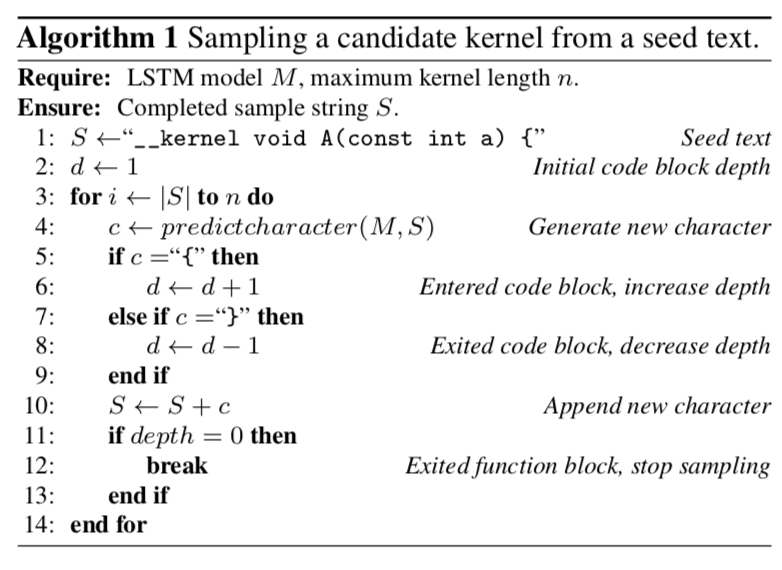
\includegraphics[scale=0.6]{Algorithm.png}
 	\end{center}
 \end{figure}\\
  \indent By using a larger number of training examples it was observed in \cite{sixth} that, the Feature F3 drawn from \cite{second} (presented in Table 1 of this report) was sparse for many programs. This was due to the nature of the training set examples in the NPB training suite \cite{nasbenchmark}. To counter this problem, \cite{sixth} then used raw feature values (like the local emery access, global memory access and average number of work items per kernel) and the combined feature values in the training set. Another drawback in the training set of \cite{second} was the absence of differentiating features in the case of branching code. This was again due to the nature of code in the NAS benchmark which was used for the training set in \cite{second}. To counter this problem a new feature was added, which is a count of the branching operations in the kernel.  The modification to the features helped to further improve the performance on an average by around 4$\times$ (5.04 on NVIDIA and 3.56 on AMD).\\
  \indent From the research in \cite{sixth} it can be observed that the hand-picked features despite being chosen by domain experts (the compiler writer in \cite{second}) had room for further improvement. This was achieved by working on the idea of expanding the dataset used for the training. However, it should be noted that human intervention was still required to tweak the features. \cite{sixth} did not automate the process of feature extraction. In fact, it's purpose was to obtain a method of generating a larger dataset that can be used for the training. Weakness in the features was detected by considering the larger dataset.
  \subsubsection{Using Deep Learning to achieve complete automation}
   In \cite{first}, the training features are learned over raw code by neural networks. The neural network constructs the internal code representation and learns code optimization. This process essentially eliminates the process of manual feature selection and hence, making the process of feature selection cheaper and much faster. The advantage of learning on the source code is that, the solution is not tied to any specific platform or compiler. The process of feature learning and prediction (CPU/GPU) involves the following stages.\\
   \indent The target code is first fed to a code rewriter which also performs the code transformations stated in \cite{sixth}. This stage removes the comments (semantically irrelevant information) from the target program and ensures trivial code differences like variable names do not affect the learned model. \\
   \indent The output from the source rewriter is then fed to the language model which converts the source code into a vector of fixed length, capturing the code properties and structure.  The source code is encoded as a sequence of integers using the language model developed in \cite{first}.  This language model is a hybrid of the character model in \cite{sixth} and vocabulary based on tokens model in \cite{token}. The keywords in the OpenCL language are assigned unique integers and the literals are encoded at character level. For example in \cite{first} `void' is encoded with the integer 3 and the literal 0 is mapped to `0' and encoded with the integer 23. The encoded source code is then mapped to vector embeddings.\\
   \indent Several OpenCL programs are encoded this way and along with the training labels (CPU/GPU) serve as the training set for the neural network. The neural network architecture consists of a two layer LSTM (Long Short Term memory) form of Recurrent Neural Network. The output of the 2 layer LSTM is a single vector that covers the entire code sequence. This step is the equivalent of finding features by domain experts in \cite{second}. The output of the 2 layer LSTM is then concatenated with auxiliary inputs (dynamic values which cannot be determined from the static code features) like work group size and data size. The concatenated vector is then fed through a deep neural network connected to two outputs, one depicting the CPU and the other a GPU. The structure of the neural network is depicted in figure 3 (a) in section 2.2.3. This model is evaluated using a 10 fold cross-validation technique \cite{tenfold}. When compared to \cite{second}, the model developed in \cite{first} had achieved a speedup of 3.34$\times$ in AMD and 1.41$\times$ in NVIDIA.\\
   \indent On comparing to the approach adopted in the previous section``Improving performance by synthesizing benchmarks". \cite{sixth} had achieved a speedup of 3.56$\times$ on AMD and 5.04$\times$  on NVIDIA. This is greater than the speedup achieved in this section which is, 3.34$\times$ in AMD and 1.41$\times$ in NVIDIA. However, the salient points to consider in this case is \cite{sixth} still required human effort to decide the features. It was aimed at improving the size of the training set for the CPU/GPU problem. \cite{first} has achieved the speedup without including the expanded training set and was trained on the same OpenCL programs that \cite{second} was trained on. The neural network approach totally eliminates the process of feature selection which requires an in-depth domain knowledge. This is one of the greatest merits of the method, devised in \cite{first}.\\
   \indent Future work in this specific research could be to use the expanded training set developed in \cite{sixth} to train the neural network method developed in \cite{first}. The performance of this model can then be used to compare the performance of the machine learning model in \cite{second}.
   \subsection{Task 2: Thread Coarsening for Graphic Processors}    
      \indent\indent Thread coercion is the process of merging together two or more parallel threads in a GPU. The challenge in this task is, to choose the optimal number of threads to coerce such that the execution of redundant instructions is avoided while still leveraging the power of parallelism. The solution to this problem tackles over-parallelism at the thread level.
  \subsubsection{Understanding thread coercion and its effects}
  The research \cite{threadseminal}, studies the effects of thread coercion and mentions the importance of choosing the right number of threads to coerce. This is because as per \cite{threadseminal} thread coercion removes instructions that are redundant. The coercing factor is not only specific to an application but also to the hardware on which it is run. This fact is supported by empirical evidence in Figure 2.
   \begin{figure}[h!]
  	\caption{Image obtained from \cite{threadseminal}}
  	\begin{center}
  	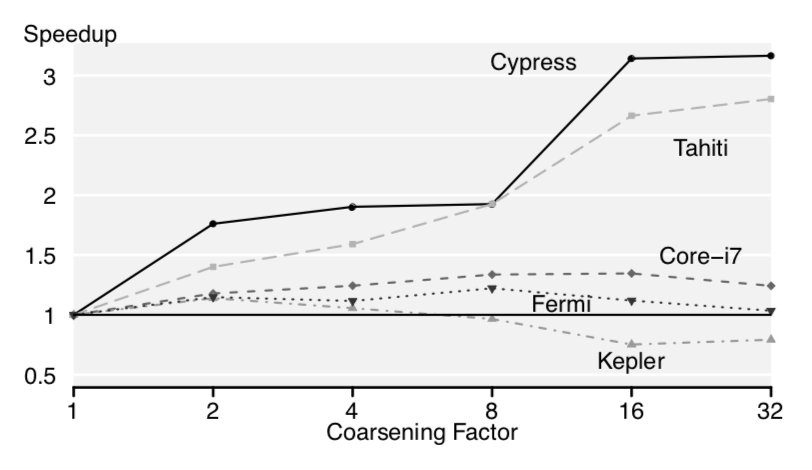
\includegraphics[scale=0.6]{Thread_Coercion.png}
  	  	\end{center}
  \end{figure}\\
  \indent Figure 2 depicts the speedup of application (finding the transpose of a matrix) on various hardware and with varying thread coarsening factors. The Cypress and Tahiti are AMD GPUs, Fermi and Kepler are NVIDIA GPUs and Core-i7 is an Intel CPU \cite{threadseminal}. From the figure 2 it can be deduced that while increasing the thread coercion factor has a positive effect on certain hardware like Cypress, on Kepler increasing the thread coercion beyond 2 has a negative effect and on Fermi the optimal coercion factor is 8. Hence, it can be concluded that thread coercion factor depends not only on the application itself but also on the hardware on which it is run on. To apply thread coercion, \cite{threadseminal} first identifies divergent instructions. These instructions are those that have different behavior in different threads (processing elements) \cite{divergence}. Clones of the divergent instructions are then created and thread coarsening is then applied. Using regression trees, \cite{threadseminal} studies independently each of the hardware (Kepler, Fermi, Cypress, Tahiti, and AMD) and the effect of important parameters like the loads, branches and so on in an application, in relation to the thread coarsening factor. It was seen that for hardware like Fermi, Kepler and Tahiti the most important factor was the load operation, for Cypress it was ALU packing and for Core-I7 it was vector instructions.\\
  \indent It can be concluded from the study in \cite{threadseminal} that, the optimal thread coercion factor depends on the application and hardware it is run on. By observing the results from the regression trees in \cite{threadseminal}, it can be further concluded that different parameters in an application have varying levels of importance across different hardware. These different parameters are affected differently by the thread coercion and hence this justifies the observations in Figure 2. To determine the optimal thread coercion factor, code versions with varying levels of thread coercion have to be tested to arrive at the optimal number of threads to coerce. 
  \subsubsection{Automatic thread coercion}
  \indent\indent In \cite{threadautomatic}, neural networks are used to determine the number of threads to coerce. The neural network is trained in 2 phases. In phase 1 of the training phase, static code features decided by the domain expert are collected from a large number of OpenCL programs. These features include the number of loads, stores, branches, divergent instructions and so on. In phase 2 of the training phase, different versions of the OpenCL programs are run with coarsening factors in the range of 2,4,8 16 and 32. A binary training output records if coarsening improved the performance.  This 5 member tuple binary training output, together with the features comprise of the training set for the neural network.\\
  \indent To determine the coarsening factor for an unseen program, the static code features are fed to the neural network to determine if coarsening should be applied. In case the output from the neural network is yes, then the coarsened version of the program is tested on the neural network. This process is repeated iteratively until an optimal coarsening value is obtained. This can be identified by the fact that, beyond the optimal point, coarsening leads to performance degradation. As per \cite{threadautomatic}, there is a performance improvement of 1.11 times on NVIDIA GPU and 1.33 times on AMD GPU.
  \subsubsection{Using Deep Learning  and Transfer Learning to achieve complete automation}
  \indent\indent Similar to the process described in the section ``Using Deep Learning to achieve complete automation'' (section 2.1.4), the source code is fed to a target rewriter and the output from source rewriter is fed through the same language model developed in \cite{first} to obtain a fixed length vector representation of the source code. The only difference, in this case, is that the training examples are different and there are no auxiliary inputs concatenated with the vector. Also, the neural network has 6 outputs (1,2,4,8,16,32) instead of 2 (CPU,GPU). The following figure (Figure 3) encapsulates these differences, wherein the figure (a) is the neural network structure for the CPU/GPU task and the figure (b) is the neural network structure for the thread coarsening task.
      \begin{figure}[h]
  	\caption{Image obtained from \cite{first}}
  	\begin{center}
  		\includegraphics[scale = 0.6]{Neural_a.png}
  	\end{center}
  \end{figure}\\
  \indent As per the experimental results, this setup achieved an average performance gain of 1.06$\times$, when compared to the  model developed in \cite{threadautomatic}. According to \cite{first} the performance gain is not much because of the small training set used in \cite{threadautomatic} which consists of only 17 programs. The model built in \cite{first} for the thread coercion problem is also trained on just these 17 programs. One way to tackle this problem is by using an expanded training set. However, \cite{first} uses a different strategy. It uses the method of transfer learning.\\
  \indent According to \cite{first} using transfer learning, it is possible to improve the accuracy of the thread coercing task. This is because in the two tasks (CPU/GPU, thread coercion) the neural network developed in \cite{first} is used to learn the code structure. According to \cite{first}, since for both tasks the neural network has the similar input which is the OpenCL code, the weights learned in the layers near input will be useful for other tasks where the neural network has similar inputs. Hence the weights learned from the first two LSTM layers of the CPU/GPU task, were transferred to the first two LSTM layers in the neural network for the task of thread coercion. According to \cite{first} there was an average of 12 percent improvement in the speedup when compared to that obtained in \cite{threadautomatic}. Hence, transfer learning helps in the improvement of performance in the thread coercion task.
 The major advantage of this method is that there is no human effort required for the feature construction and the performance gain is obtained at little extra effort once the neural network is constructed and the weights have been learned.
  
  \section{Summary and Conclusion}
\indent \indent For the CPU/GPU task, while \cite{first} uses neural networks to learn the features, it still uses the limited training examples used in \cite{second}. The experimental results prove that \cite{first} gives an improved performance gain (speedup) when compared to \cite{second}. However, it should be possible to obtain an even more improved performance  by expanding the training set. The researchers had previously relied upon readily available benchmarks for training and testing. \cite{sixth} presents a method of generating developer-like code from a machine. This can be used for expanding the training set.\\
   \indent Future work could be to first expand the training set and then record the performance improvement when compared to \cite{second}. Another very important work that should be done is to create a training set of very large size using \cite{sixth}, that should be standardized across the scientific community and will be a superset of all the benchmarks that exist. This will genuinely help future researchers in this field, by  eradicating the problem of data sparsity. It will serve as a standard benchmark on which all future models, can be built and tested on. \\ \indent For the thread coercion task, a comparative study can be set up which involves a combination of expanding the training set and using transfer learning.
    



%                Now build the reference list
\bibliographystyle{unsrt}   % The reference style
%                This is plain and unsorted, so in the order
%                they appear in the document.


\bibliography{main}       % bib file(s).

\end{document}

